\chapter{Аналитическая часть}

В данной части проводится анализ существующих алгоритмов, математических моделей и программных технологий, применяемых для решения комплексной задачи трёхмерного моделирования движения автомобиля в условиях городской среды. Основной целью аналитической части является обоснованный выбор методов визуализации, удаления невидимых поверхностей, расчета освещенности, построения теней и алгоритмической организации движения объекта по кратчайшему маршруту.

\section{Формализация объектов синтезируемой сцены}

Трёхмерная сцена представляет собой модель участка городской территории, включающую в себя здания, дорожную сеть и прочие элементы окружающей среды. Все геометрические построения и расчеты производятся в единой декартовой системе координат. Для корректной визуализации и взаимодействия объектов необходимо определить состав элементов сцены и способ их математической формализации в виде структур данных.

\begin{enumerate}
	\item \textbf{Дороги.} Дороги представляют собой совокупность полигонов, образующих плоскость, по которой осуществляется движение. Для целей логического моделирования движения автомобиля дорожная сеть дополнительно описывается двумя двумерными массивами: матрицей проходимости, определяющей статические препятствия и свободные участки, и матрицей разрешённых направлений, которая задает правила движения на каждом конкретном участке. Геометрически дорога описывается набором вершин и граней с наложенными текстурами, имитирующими дорожное покрытие.
	
	\item \textbf{Здания.} Здания моделируются как набор простейших геометрических примитивов, таких как параллелепипеды и призмы различной конфигурации. Каждое здание описывается через полигональную сетку, состоящую из списков вершин в трехмерном пространстве и списков граней, соединяющих эти вершины. Для повышения визуальной реалистичности используется текстурирование фасадов изображениями окон, дверей и материалов стен.
	
	\item \textbf{Малые архитектурные формы.} Малые архитектурные формы, включающие скамьи и фонарные столбы, моделируются как набор простейших геометрических примитивов. Каждое объект описывается через полигональную сетку, состоящую из списков вершин в трехмерном пространстве и списков граней, соединяющих эти вершины. Для повышения визуальной реалистичности используется текстурирование поверхностей.
	
	\item \textbf{Автомобиль.} Автомобиль является ключевым динамическим объектом сцены. Его геометрическая модель формируется из сложного набора вершин, рёбер и граней, образующих кузов и колеса. Положение автомобиля в пространстве однозначно задаётся вектором координат его геометрического центра и матрицей поворота, определяющей текущую ориентацию корпуса относительно осей координат. Модель поддерживает аффинные преобразования для имитации езды.
	
	\item \textbf{Источник света.} Источник света описывается вектором направления световых лучей и интенсивностью излучения. В данной задаче используется модель бесконечно удалённого источника света, имитирующего солнечное освещение. Особенностью данной модели является допущение, при котором все световые лучи считаются параллельными друг другу, что упрощает расчеты теней и освещенности для всех объектов сцены.
	
	\item \textbf{Камера.} Камера представляет собой виртуального наблюдателя, через которого пользователь воспринимает трехмерную сцену. Её параметры включают положение в мировых координатах, точку направления взгляда и вектор ориентации верха камеры. Все объекты сцены визуализируются путем перевода их координат в систему отсчета камеры с последующей перспективной проекцией на плоскость экрана.
\end{enumerate}

Для хранения геометрической информации об объектах сцены используется полигональное представление. При таком подходе каждая поверхность описывается множеством вершин с уникальными координатами и списком граней, которые ссылаются на индексы этих вершин. Данный формат храения данных позволяет эффективно применять алгоритмы растеризации и трансформации \cite{rogers_base}.

\section{Анализ алгоритмов удаления невидимых поверхностей}

Одной из фундаментальных задач трёхмерной визуализации является устранение невидимых поверхностей. Суть задачи заключается в определении того, какие части объектов перекрываются другими объектами с точки зрения наблюдателя и, следовательно, не должны выводиться на экран монитора.

\subsection{Алгоритм обратной трассировки лучей}

Основная идея метода состоит в моделировании процесса распространения света в обратном направлении --- не от источников, а от наблюдателя к объектам сцены \cite{shikin_boreskov}. Поскольку считается, что наблюдатель расположен на бесконечности вдоль положительного направления оси~$z$, все испускаемые им лучи можно считать параллельными этой оси. Для каждого пикселя экрана формируется первичный луч, выпущенный из камеры.

Далее для данного луча определяется пересечение со всеми объектами. Из всех найденных точек выбирается та, которая имеет максимальную координату~$z$, то есть находится ближе всего к наблюдателю.

Для расчетов освещения из точки пересечения проводятся вторичные лучи, направленные к каждому источнику света. Если на пути такого луча обнаруживается непрозрачный объект, точка считается находящейся в тени. В противном случае учитывается вклад освещения.

\textbf{Преимущества:} метод обеспечивает высокую степень реалистичности, так как опирается на физически корректное моделирование распространения света.

\textbf{Недостатки:} метод является вычислительно затратным, точное определение пересечений лучей с геометрическими объектами требует решения сложных математических уравнений, что существенно снижает скорость при программной реализации.


\subsection{Алгоритм Робертса}

Данный алгоритм работает в объектном пространстве и предназначен для обработки исключительно выпуклых тел, реализуется этот алгоритм в три этапа \cite{rogers_base}. 

На первом этапе формируется исходная матрица $V$, содержащая информацию о каждой грани многогранника. Размерность матрицы составляет $4 \times n$, где $n$ -- количество граней. Каждый столбец соответствует коэффициентам уравнения плоскости вида $ax + by + cz + d = 0$, описывающей конкретную грань:

\[
V = \begin{pmatrix}
	a_1 & a_2 & \dots & a_n \\
	b_1 & b_2 & \dots & b_n \\
	c_1 & c_2 & \dots & c_n \\
	d_1 & d_2 & \dots & d_n
\end{pmatrix}
\tag{1}
\]

Требуется обеспечить корректность формирования матрицы: любая точка внутри тела должна находиться с положительной стороны относительно каждой грани. Если для какой-либо грани это условие не выполняется, соответствующий столбец матрицы умножается на $-1$. Для проверки используется внутренняя точка тела, координаты которой можно получить усреднением координат всех его вершин.

На втором этапе выполняется определение рёбер, экранируемых самим телом. Задаётся вектор направления взгляда $\mathbf{E} = \{0, 0, -1, 0\}$. Для выявления невидимых граней вычисляется произведение:

\[
\mathbf{R} = \mathbf{E} \cdot \mathbf{V}
\]

Компоненты результирующего вектора $\mathbf{R}$, имеющие отрицательные значения, соответствуют невидимым граням.

Третий этап предполагает удаление рёбер, перекрываемых другими объектами сцены. Для проверки видимости конкретной точки на ребре строится луч, соединяющий позицию наблюдателя с анализируемой точкой. Точка является невидимой, если на пути луча встречается рассматриваемое тело как препятствие. Факт пересечения лучом тела определяется условием нахождения луча с положительной стороны относительно плоскости каждой грани данного тела.


\textbf{Преимущества:} обеспечение высокой точности результата, достигаемой за счёт работы в объектном пространстве, что позволяет выполнять вычисления непосредственно с математическим описанием тел.

\textbf{Недостатки:} высокая вычислительная трудоёмкость алгоритма, составляющая $O(n^2)$, где $n$ — количество объектов в сцене. Также недостатком является требование к геометрии: все тела должны быть строго выпуклыми, что накладывает необходимость проведения дополнительных проверок корректности их описания и разбиения невыпуклых объектов на выпуклые части.


\subsection{Алгоритм построчного сканирования с использованием буфера глубины. Алгоритм Z-буфера}

Алгоритм Z-буфера относится к методам, работающим в пространстве изображения и служит для определения видимости фрагментов сцены. Его идея представляет собой расширение концепции буфера кадра за счёт добавления второго массива данных --- буфера глубины, в котором для каждого пикселя хранится значение координаты $z$ \cite{rogers_base}.

\textbf{Основной принцип работы:} перед началом рендеринга буфер кадра заполняется значениями фона, а буфер глубины инициализируется минимальными возможными значениями $z$. Далее сцена обрабатывается построчно. Для каждого активного многоугольника внутри текущей строки вычисляются границы его видимой области. Затем для каждого пикселя внутри этих границ интерполируется его значение глубины. Полученное значение сравнивается с соответствующей записью в буфере глубины: если новый фрагмент расположен ближе к наблюдателю, чем уже записанный, выполняется закраска пикселя и обновление буфера глубины. Если же глубина больше, пиксель игнорируется. Принцип работы алгоритма представлен на рисунке \ref{fig:z_buffer_concept}.

\begin{figure}[H]
	\centering
	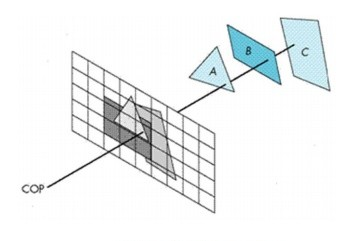
\includegraphics[width=0.6\textwidth]{img/z_buffer_concept}
	\caption{Принцип работы Z-буфера: сохранение глубины ближайшего фрагмента}
	\label{fig:z_buffer_concept}
\end{figure}

\textbf{Преимущества:} алгоритм не требует предварительной сортировки полигонов и позволяет выводить геометрические объекты в произвольном порядке. Благодаря этому Z-буфер эффективно обрабатывает сцены с большим количеством перекрывающихся объектов и корректно определяет ближайшие фрагменты. Сложность алгоритма масштабируется линейно с количеством обрабатываемых пикселей, что делает его удобным для применения в растровых графических системах.

\textbf{Недостатки:} метод требует выделения дополнительной памяти под буфер глубины, что может быть критично при высоких разрешениях. Также Z-буфер затрудняет корректную обработку прозрачных поверхностей, так как для них необходима сортировка фрагментов по глубине. Устранение ступенчатости контуров и реализация полупрозрачности требуют дополнительных процедур.


\subsection{Обоснование выбора}

Для реализации выбран алгоритм построчного сканирования с использованием буфера глубины. В отличие от алгоритма Робертса, данный подход корректно обрабатывает пересекающиеся объекты и не зависит от возможных ошибок в топологии моделей. По сравнению с методом трассировки лучей, выбранный алгоритм проще и эффективнее поддается векторизации на основе матричных операций, что позволяет обеспечить необходимую производительность.


\section{Анализ методов закрашивания}

Закрашивание определяет математический способ вычисления цвета каждой точки поверхности с учётом свойств материала и условий освещения. Выбор метода напрямую влияет на реалистичность и скорость рендеринга. Сравнение визуальных результатов различных методов представлено на рисунке \ref{fig:shading_models}.

\begin{figure}[H]
	\centering
	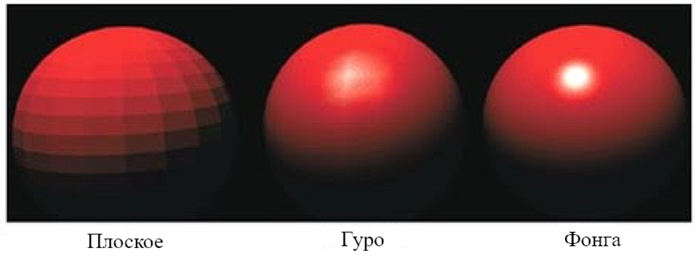
\includegraphics[width=0.8\textwidth]{img/shading_models}
	\caption{Сравнение методов закрашивания: Плоское, Гуро, Фонга}
	\label{fig:shading_models}
\end{figure}

\subsection{Плоское закрашивание}

При использовании данного метода для каждой грани вычисляется нормаль. Интенсивность освещённости рассчитывается по закону Ламберта как произведение интенсивности источника света на косинус угла падения лучей. Весь полигон целиком закрашивается одним цветом с рассчитанной интенсивностью, что придает объектам граненый вид. \cite{rogers_base}

\textbf{Преимущества:} метод требует минимальных вычислительных затрат, так как расчет освещения выполняется один раз на целый полигон, а не для каждого пикселя в отдельности.

\textbf{Недостатки:} основным минусом является дискретность получаемого изображения. При аппроксимации криволинейных поверхностей отчетливо видны границы между смежными полигонами, из-за чего теряется гладкость формы. Этот визуальный дефект усиливается оптической иллюзией. Кроме того, метод не позволяет корректно отображать зеркальные блики: поскольку нормаль постоянна для всей грани, блик либо заливает полигон целиком, либо отсутствует полностью.

\subsection{Закрашивание по методу Гуро}

Метод Гуро основан на линейной интерполяции интенсивности освещения по поверхности полигона. Процесс состоит из трех этапов: сначала вычисляются нормали в вершинах, затем для каждой вершины рассчитывается цвет согласно выбранной модели освещения, и, наконец, при растеризации цвет внутренних пикселей вычисляется путем билинейной интерполяции цветов вершин \cite{rogers_base}.

\textbf{Преимущества:} метод позволяет скрыть граненую структуру модели, создавая иллюзию гладкой поверхности. При этом он относительно вычислительно эффективен, так как сложные расчеты освещения (с векторами и косинусами) производятся только для вершин, количество которых значительно меньше количества пикселей.

\textbf{Недостатки:} основной проблемой метода является потеря зеркальных бликов, если они попадают в центр полигона, а не на вершину, то блик «размазывается» или исчезает при интерполяции.

\subsection{Закрашивание по методу Фонга}

Метод Фонга предполагает интерполяцию вектора нормали к поверхности для каждого пикселя. Вместо готового цвета, между вершинами интерполируются компоненты вектора нормали. Затем для каждого пикселя, используя полученную интерполированную нормаль, производится полный расчет освещенности по выбранной модели. \cite{rogers_base}

\textbf{Преимущества:} обеспечивает наиболее реалистичное отображение криволинейных поверхностей среди локальных моделей освещения. Метод корректно воспроизводит четкие зеркальные блики в любой точке полигона и дает очень плавные градиенты освещенности.

\textbf{Недостатки:} крайне высокая вычислительная сложность. Необходимость нормализовать вектор и вычислять скалярные произведения для каждого пикселя экрана создает колоссальную нагрузку на процессор. При программной реализации без использования GPU этот метод часто приводит к неприемлемо низкому количеству кадров в секунду (FPS) для сцен с большим количеством объектов.

\subsection{Обоснование выбора}
Выбран метод плоского закрашивания. Поскольку рендеринг выполняется на центральном процессоре без использования графического ускорителя, применение более сложных методов приведет к значительному снижению частоты кадров. Простое закрашивание обеспечивает достаточную наглядность геометрии городских зданий, состоящих преимущественно из плоских поверхностей, при максимальной производительности системы.

\section{Построение теней}
Тени являются важным элементом восприятия глубины, позволяющим зрителю определить взаимное расположение объектов в пространстве.

\subsection{Теневые объёмы}

Теневые объёмы (Shadow Volumes) — это геометрический метод построения теней, который создаёт виртуальные объёмы за объектами, внутри которых точки сцены находятся в тени. Идея метода заключается в том, чтобы определить силуэтные грани объектов относительно источника света и вытянуть их вдаль, формируя объём, через который можно проверить, какие пиксели будут затенены. Для этого обычно используется буфер трафарета, позволяющий классифицировать каждый пиксель как освещённый или находящийся в тени \cite{ShadowVolumeCode}.  

\textbf{Преимущества:} метод обеспечивает высокую точность построения теней с чёткими границами, не зависит от масштаба или расстояния до камеры, а также не требует специальных параметров для устранения артефактов самозатенения. Использование видеокарты позволяет значительно ускорить обработку и сделать метод применимым к сложным сценам.  

\textbf{Недостатки:} высокая вычислительная нагрузка, особенно при сложной геометрии, требует значительных ресурсов процессора. В реальных проектах часть вычислений обычно переносится на GPU, что делает метод более эффективным, но сохраняет высокие требования к аппаратуре. Также с помощью этого метода сложно реализовать тени для полупрозрачных объектов.


\subsection{Метод карт теней}

Алгоритм построения теней с использованием Z-буфера является двухпроходным \cite{williams_shadows}. На первом этапе сцена визуализируется с позиции источника света, при этом сохраняется только информация о глубине поверхностей в специальный буфер. На втором этапе сцена рендерится с точки зрения наблюдателя, а координаты каждой видимой точки преобразуются в пространство света и проверяются на видимость относительно источника. Если точка оказывается невидимой для света, она затемняется, формируя соответствующую тень. Такая реализация позволяет корректно отображать тени на кривых поверхностях и учитывать самозатенение объектов, при этом все дополнительные вычисления ведутся в пространстве изображения, что делает алгоритм относительно универсальным и независимым от сложности сцены. Пример обработки сцены представлен на рисунке \ref{fig:shadow_mapping}

\begin{figure}[H]
	\centering
	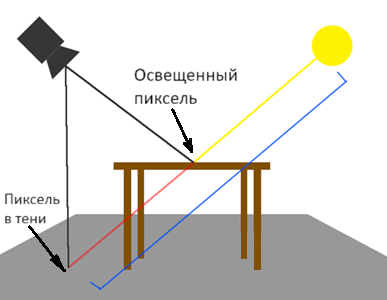
\includegraphics[width=0.7\textwidth]{img/shadow_mapping_concept}
	\caption{Двухпроходный алгоритм построения карт теней}
	\label{fig:shadow_mapping}
\end{figure}

\textbf{Преимущества:} универсальность метода позволяет теням корректно ложиться на любые объекты независимо от их формы, а также автоматически поддерживает самозатенение \cite{learnopengl_shadows}.

\textbf{Недостатки:} качество теней напрямую зависит от разрешения карты глубины: при его недостатке края теней становятся пикселизированными. Из-за дискретности буфера часто возникают артефакты, для устранения которых требуется подбор параметра смещения, что может привести к визуальному отрыву тени от объекта. Кроме того, необходимость двукратной отрисовки геометрии существенно увеличивает вычислительную нагрузку.

\subsection{Обоснование выбора}
Выбран метод карт теней. Проекционные тени недостаточно реалистичны для городской среды, где тени могут падать на стены зданий и другие машины. Метод карт теней идеально интегрируется в выбранный конвейер с использованием буфера глубины, позволяя использовать схожие алгоритмы растеризации для обоих проходов визуализации.

\section{Организация движения автомобиля и поиск пути}

Для реализации автоматического движения автомобиля необходимо выбрать алгоритм поиска кратчайшего пути на графе дорожной сети.

\subsection{Алгоритм Дейкстры}

Алгоритм Дейкстры предназначен для поиска кратчайших путей от одной вершины графа до всех остальных. Он работает с графами, имеющими неотрицательные веса ребер. Алгоритм последовательно выбирает вершину с наименьшей меткой расстояния и релаксирует ребра, исходящие из неё \cite{algorithmica_dijkstra}.

\textbf{Преимущества:} гарантированно находит кратчайший путь.

\textbf{Недостатки:} в случае равномерной сетки, где веса всех ребер равны единице, алгоритм Дейкстры выполняет избыточные операции с очередью с приоритетом, что делает его менее эффективным по сравнению с более простыми методами обхода.

\subsection{Муравьиный алгоритм}

Муравьиный алгоритм является метаэвристическим методом оптимизации, вдохновлённым поведением настоящих муравьёв при поиске кратчайших путей к источнику пищи. Алгоритм использует виртуальных <<муравьёв>>, которые перемещаются по графу, откладывая и следуя феромонным следам. С течением времени наиболее успешные пути накапливают больше феромонов, что повышает вероятность их выбора последующими муравьями \cite{donntu_murzin_muravyinye_algoritmy}.

\textbf{Преимущества:} способность находить хорошие решения для сложных комбинаторных задач, устойчивость к локальным минимумам, возможность параллельного выполнения.

\textbf{Недостатки:} относительно низкая скорость сходимости для больших графов, необходимость подбора параметров (скорость испарения феромонов, влияние феромонов и эвристики), результаты могут быть стохастически изменчивыми и требовать многократного запуска для получения стабильного решения.

\subsection{Волновой алгоритм}

Волновой алгоритм является вариацией поиска в ширину на графе. Он работает путем распространения волны от стартовой точки во все стороны равномерно, рисунок \ref{fig:wave_algo}. Поскольку дорожная сеть представлена в виде сетки с одинаковыми весами ребер, волна гарантированно находит кратчайший путь \cite{wave_suvitruf}.

\begin{figure}[H]
	\centering
	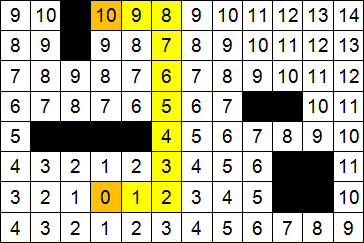
\includegraphics[width=0.5\textwidth]{img/wave_algo}
	\caption{Распространение волны в алгоритме поиска пути на сетке}
	\label{fig:wave_algo}
\end{figure}

\textbf{Преимущества:} идеально подходит для дискретных сеток и лабиринтов. Легко модифицируется для учета запрещенных направлений движения путем проверки матрицы смежности или матрицы направлений.

\textbf{Недостатки:} Алгоритм является «слепым», то есть он исследует пространство равномерно во все стороны, не учитывая направление на целевую точку. Это приводит к посещению большого количества лишних вершин и снижению производительности на картах большого размера по сравнению с эвристическими алгоритмами.

\subsection{Выбор алгоритма поиска пути}

Для реализации выбран модифицированный волновой алгоритм для ориентированного графа.

\textbf{Обоснование:} дорожная сеть в проекте представлена в виде клеточной матрицы, где расстояние между соседними клетками всегда равно единице. В таких условиях волновой алгоритм является оптимальным решением, гарантирующим нахождение кратчайшего пути. Кроме того, использование дополнительной матрицы направлений позволяет легко интегрировать в алгоритм правила дорожного движения, запрещая распространение волны против разрешенного потока.

\section{Текстурирование}

Для повышения визуальной реалистичности сцены без увеличения сложности геометрии используется метод UV-развертки текстур. Этот метод позволяет отображать двумерное изображение (текстуру) на трёхмерной поверхности модели. Каждой вершине треугольника присваиваются координаты $(u, v)$, которые указывают на соответствующую точку на текстуре. В процессе растеризации треугольника для каждого пикселя вычисляются интерполированные значения этих координат, что позволяет корректно отображать текстуру на поверхности с учётом её формы и ориентации \cite{digital_razor_uv_mapping}.

UV-развертка особенно полезна для сложных моделей, где прямое наложение текстуры было бы невозможным или привело бы к значительным искажениям. Она обеспечивает точное соответствие текстурных деталей геометрии объекта и позволяет создавать реалистичные материалы без увеличения количества полигонов. 

Метод UV-развертки обеспечивает оптимальный баланс между качеством визуализации и производительностью. Он позволяет достигать высокой скорости рендеринга и чёткости текстур, не нагружая центральный процессор, что особенно важно для рендеринга при ограниченных ресурсах. Основные ограничения метода включают возможную пикселизацию при увеличении масштаба текстуры и необходимость аккуратного построения UV-развертки для минимизации растяжений и швов на поверхности модели.


\section{Выводы по аналитической части}

В ходе всестороннего анализа предметной области и существующих алгоритмов компьютерной графики был сформирован стек методов.

\begin{enumerate}
	\item \textbf{Визуализация:} выбран алгоритм с использованием Z-буффера, так как он обеспечивает корректное отображение геометрии и устойчив к ошибкам моделирования.
	\item \textbf{Тени:} выбран метод карт теней, который обеспечивает построение реалистичных динамических теней от объектов любой формы.
	\item \textbf{Освещение:} выбрано плоское закрашивание по модели Ламберта, предоставляющее оптимальный баланс между качеством визуализации объёма и скоростью работы на центральном процессоре.
	\item \textbf{Текстурирование:} выбран метод с использованием UV-развертки и выборкой ближайшего соседа, что позволяет повысить детализацию сцены при минимальных вычислительных затратах.
	\item \textbf{Логика движения:} выбран волновой алгоритм на ориентированном графе, позволяющий строить корректные маршруты с учётом правил дорожного движения и односторонних дорог.
\end{enumerate}

Сформированный набор методов и алгоритмов позволяет создать систему моделирования движения автомобиля.